\documentclass[pdf,dvipsnames,aspectratio=169]{beamer}
\usetheme{Madrid}

\usepackage{xkeyval}
\usepackage{todonotes}
\presetkeys{todonotes}{inline}{}
\usepackage{graphicx}
\usepackage{subfig}
\usepackage{multimedia}                % include movies
\usepackage{breqn}                     % break equations automatically
\usepackage{cancel}                    % cancel out text/equations
\usepackage{color}                     % colored font
\usepackage{wasysym}                   % smiley (smiling face)
\usepackage[absolute,overlay]{textpos} % to put a box in front of text
\usepackage{mathtools}                 % use dcases to display nice fractions in cases
\usepackage{multicol}                  % split tof
\usepackage[figurename=Fig]{caption}
\usepackage{tcolorbox}
\usepackage{calc}
\usepackage{multirow}
\usepackage{dcolumn}
\usepackage{adjustbox}

\usepackage{hyperref}
% \hypersetup{
% 	pdftitle   = {Brown bag seminar},
% 	pdfauthor  = {Pablo Botas},
% 	pdfcreator = {Pablo Botas},
% 	colorlinks = true,
% 	linkcolor  = cyan,
% 	linktoc    = black,
% 	citecolor  = black,
% 	filecolor  = black,
% 	urlcolor   = black,
% 	baseurl={}
% 	}

\setlength\abovecaptionskip{0pt}

\usepackage{pgfpages}
% \setbeameroption{show notes on second screen}
\beamertemplatenavigationsymbolsempty
\setbeamertemplate{footline}[frame number]

\newcommand\blfootnote[1]{%
	\begingroup
	\renewcommand\thefootnote{}\footnote{#1}%
	\addtocounter{footnote}{-1}%
	\endgroup
}

% SEE http://latexcolor.com/
\definecolor{flame}{rgb}{0.89, 0.35, 0.13}
\definecolor{iceberg}{rgb}{0.44, 0.65, 0.82}
\definecolor{inchworm}{rgb}{0.7, 0.93, 0.36}
\definecolor{brandeisblue}{rgb}{0.0, 0.44, 1.0}

\AtBeginDocument{\setlength\abovedisplayskip{0pt}}
\AtBeginDocument{\setlength\belowdisplayskip{10pt}}
\AtBeginDocument{\setlength\abovedisplayshortskip{0pt}}
\AtBeginDocument{\setlength\belowdisplayshortskip{0pt}}


\begin{document}
\title[Assessing the need and feasibility for online plan adaptation based on daily CBCT of head and neck proton therapy treatments]{Assessing the need and feasibility for online plan adaptation based on daily CBCT of head and neck proton therapy treatments}
\author{\texorpdfstring{P. Botas\inst{1}\inst{2}, J. Kim\inst{1}, C. Grassberger\inst{1}, B. Winey\inst{1}, H. Paganetti\inst{1} \newline{\scriptsize\url{pbotas@mgh.harvard.edu}}}{Pablo Botas}}
\institute{\inst{1}Massachusetts General Hospital and Harvard Medical School, Boston, MA \and \inst{2}Heidelberg University, Heidelberg, Germany}
\titlegraphic{\includegraphics[height=2cm]{imgs/MGHHMSLogo.pdf} \hspace*{2cm} ~%
    \includegraphics[height=2cm]{imgs/Logo_University_of_Heidelberg.pdf}
}
\date{AAPM, 59th Annual Meeting \& Exhibition}

\begin{frame}
    \titlepage
\end{frame}

% \begin{frame}
%     \todo[inline]{Free approach would allow the implementation in non-parallel vf scenarios like P1}
%     \todo[inline]{High LET at the end of range, we still have range uncertainties due to the HU to STP conversion.}
% \end{frame}

\section{Motivation}
\begin{frame}[c]{Motivation}
    \begin{columns}[c]
        \begin{column}{0.5\textwidth}
            Problem and potential solution:
            \begin{itemize}
                \item Intensity modulated Proton therapy (\textbf{IMPT}) \textbf{is sensitive} to geometry changes
                \item To increase plan quality, \textbf{margins should be reduced}
                \item \textbf{Adaptive therapy could allow margin reduction} by correcting inter-fractional geometry changes and mispositioning
                \item \textbf{Head and neck patients} are perfect candidates to benefit from the technique
            \end{itemize}
        \end{column}
        \begin{column}[c]{0.5\textwidth}
            \begin{figure}[h]
                \centering
                \includegraphics[height=0.6\textheight]{{imgs/VF}.png}
                \caption{Head and neck patient geometry changes. The original CT is green, the CBCT is red, the arrows represent the vector field, the arrow color is a representation of their length.}
            \end{figure}
        \end{column}
    \end{columns}
\end{frame}

% MENTION THAT WE EVALUATE AFTER WARPING THE CONTOURS
% Fix caption
% Add angle to axis labels
\section{The need for adaptive proton therapy}
\begin{frame}[c]{The need for adaptive proton therapy}
    \begin{columns}[c]
        \begin{column}{0.45\textwidth}
            Head \& neck patients planned without CTV margins, evaluated at different fractions:
            \begin{itemize}
                \item Reducing margins makes plans very sensitive to errors
                \item Adaptive proton therapy is needed
            \end{itemize}
            \vspace*{-0.4cm}
            \begin{figure}[h]
                \includegraphics[width=\textwidth]{{imgs/Mean.CTV.week}.pdf}
                \caption{Mean CTV dose decreases}
            \end{figure}
        \end{column}
        \begin{column}[c]{0.55\textwidth}
%             \vspace*{-0.5cm}
            \begin{figure}[h]
                \includegraphics[width=\textwidth]{{imgs/DVH.Pat.3}.pdf}
                \caption{DVHs at plan, fraction 3 and 6}
            \end{figure}
%             \vspace*{-1cm}
%             \begin{figure}[h]
%                 \centering
%                 \includegraphics[width=0.9\textwidth]{{imgs/Mean.OARs.reduced.week}.pdf}
%                 \caption{Mean dose increase of spinal cord and larynx}
%             \end{figure}
        \end{column}
    \end{columns}
\end{frame}

\section{Adaptive proton therapy ingredients: the framework}
\begin{frame}[c]{Adaptive proton therapy ingredients: the framework}
    \begin{columns}[c]
        \begin{column}{0.48\textwidth}
            \vspace*{-2mm}
            {\setbeamercolor{block title}{bg=flame, fg=black}
                \begin{block}{Cone Beam CT (CBCT)}
                    \textit{A priori} CT-based scatter correction WEPL error $< 2\%$ in head cases.\\
                    {\begin{flushright}\scriptsize\textit{Park et al., Med Phys. 2015;42(8)}, \textit{Kim et al., Phys Med Bio. 2017;62(1)}\end{flushright}}
                \end{block}}
            {\setbeamercolor{block title}{bg=iceberg, fg=black}
                \begin{block}{Image Registration: Plastimatch}
                    Rigid and deformable (DIR), GPU B-spline\\
                    {\hfill\scriptsize\textit{Shackleford et al., Phys Med Biol. 2010;55(21)}}
                \end{block}}
            {\setbeamercolor{block title}{bg=inchworm, fg=black}
                \begin{block}{Fast GPU MC: gPMC}
                    Accurate calculation engine developed with UT Southwestern.\\
                    {\hfill\scriptsize\textit{Qin et al., Phys Med Biol. 2016;61(20)}}
                \end{block}}
        \end{column}
        \begin{column}{0.5\textwidth}
            \centering
            %question mark has RGBA code ffaf0072
            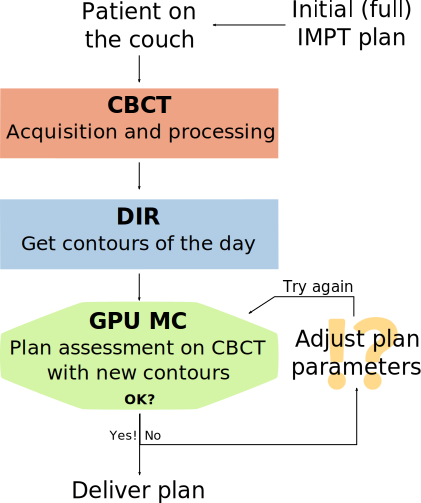
\includegraphics[width=0.8\textwidth]{{imgs/drawing}.pdf}
        \end{column}
    \end{columns}
\end{frame}

\section{Adaptation method}
\begin{frame}[c]{Adaptation method}
    \begin{columns}[t]
        \begin{column}{0.5\textwidth}
            \only<1-9>{
                A vector field (VF) from DIR links CT and CBCT.\\
                The VF is employed to:
                \begin{enumerate}
                    \item<1-> Transport contours to new geometry
                    \item<2-> Warp IMPT plan (not dose). Per spot $s_i = (x_0, y_0, E_0)$:
                    \begin{itemize}
                        \item[1:]<3-> \textbf{Raytrace} $s_i$ in CT ($r_i$)
                        \item[2:]<4-> \textbf{Probe} VF at $r_i$ coords: $v_i$
                        \item[3:]<5-> \textbf{Apply $v_i$ to $r_i$} coords: position where the $r_i$ should be in the CBCT
                        \item[4:]<6-> \textbf{Apply $v_i$ to $s$} $\rightarrow $ $s'_i = (x_0 + \Delta v_x, y_0 + \Delta v_y, E_0)_i$
                        \item[5:]<7-> \textbf{Raytrace} $s'_i$ in CBCT
                        \item[6:]<8-> \textbf{Get} $\Delta E_i$
                    \end{itemize}
                    \item<9> Spot adaptation: $(\Delta v_x, \Delta v_y, \Delta E)_i$
                \end{enumerate}
            }
            \only<10>{
                \vspace*{-8mm}
                \begin{figure}
                    \includegraphics[width=\textwidth]{imgs/plan_shifts.pdf}
                    \caption{Plan positions shifted}
                \end{figure}
                \vspace{-1.0cm}
                \begin{figure}
                    \includegraphics[width=\textwidth]{imgs/energy_shifts.pdf}
                    \caption{Energy shifts histogram.}
                \end{figure}
            }
        \end{column}
        \begin{column}{0.45\textwidth}
            \only<1-9>{\vspace{-1cm}}
            \only<10->{\vspace{-7mm}}
            \begin{figure}
                \only<1-3>{\includegraphics[height=0.8\textheight]{imgs/adaptation_method_1.pdf}}
                \only<4>{\includegraphics[height=0.8\textheight]{imgs/adaptation_method_2.pdf}}
                \only<5>{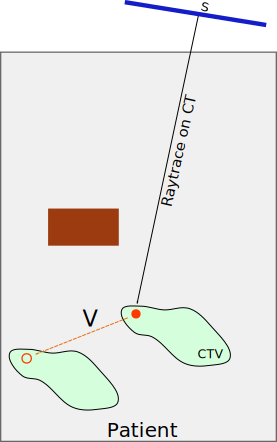
\includegraphics[height=0.8\textheight]{imgs/adaptation_method_3.pdf}}
                \only<6>{\includegraphics[height=0.8\textheight]{imgs/adaptation_method_4.pdf}}
                \only<7>{\includegraphics[height=0.8\textheight]{imgs/adaptation_method_5.pdf}}
                \only<8->{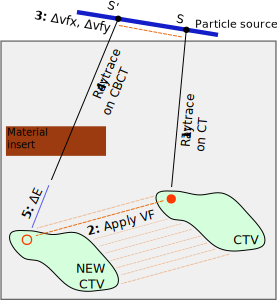
\includegraphics[height=0.8\textheight]{imgs/adaptation_method_end.pdf}}
            \end{figure}
        \end{column}
    \end{columns}
\end{frame}

\section{Methodology}
\begin{frame}[c]{Methodology}
    \begin{columns}[c]
        \begin{column}{0.45\textwidth}
            Energy layer organization is distorted by this method.\\

            Two strategies:
            \begin{itemize}
                \item {\color{brandeisblue} Free:} No constrains on the spots movement $(\Delta v_x, \Delta v_y, \Delta E)_i$
                \item {\color{brandeisblue} Rigid beams:}
                \begin{itemize}
                    \item \textit{Couch shift}: Average VF in the CTV
                    \item \textit{Range-shifter-of-the-day}: Average energy shift
                \end{itemize}
            \end{itemize}
        \end{column}
        \begin{column}{0.55\textwidth}
            \vspace*{-0.4cm}
            \begin{figure}[b!]
                \centering
                \includegraphics[width=\textwidth]{imgs/plan_energy_layer_destruction.pdf}\\
                \includegraphics[width=\textwidth]{imgs/plan_energy_layer_conservation.pdf}
                \caption{Distortion/conservation of plan energy layers}
            \end{figure}
        \end{column}
    \end{columns}
\end{frame}

%IMPT heavily exploits dose irregularities that are not captured in this method
\section{Results}
\begin{frame}[c]{Results}
    \vspace*{-0.5cm}
    \begin{columns}[c]
        \begin{column}{0.4\textwidth}
            \begin{figure}[h]
                \centering
                \includegraphics[width=0.75\textwidth]{imgs/annotated_beam_shift.png}\\
                \includegraphics[width=0.75\textwidth]{imgs/annotated_P3_F5.png}
                \caption{Adapted minus original dose. Red means more dose by adapted distribution. The shifts follow the VF (arrows). \textbf{Top:} a single spot. \textbf{Bottom:} 3 beams}
            \end{figure}
        \end{column}
        \begin{column}{0.6\textwidth}
            \begin{figure}[h]
                \begin{columns}[c]
                    \begin{column}{0.65\textwidth}
                        \includegraphics[width=\textwidth]{{imgs/DVHs_P03_week_5_SLIDES}.pdf}\\
                        \only<1>{\includegraphics[width=\textwidth]{{imgs/DVHs_P15_week_1_SLIDES}.pdf}}
                        \only<2>{\includegraphics[width=\textwidth]{{imgs/DVHs_P02_week_1_SLIDES}.pdf}}
                    \end{column}
                    \begin{column}{0.35\textwidth}
                        \only<1>{\caption{Example DVHs with {\color{green} original}, {\color{blue}adapted}, and {\color{red}non-adapted} plan.\\
                                \textbf{Top:} some improvement, steeper DVH, but plan quality not restored\\
                                \textbf{Bottom:} Little improvement.}}
                        \only<2>{\caption{Example DVHs with {\color{green} original}, {\color{blue}adapted}, and {\color{red}non-adapted} plan.\\
                                \textbf{Top:} considerable improvement, steeper DVH, but plan quality not restored\\
                                \textbf{Bottom:} VF divergences make adapted plan worse.}}
                    \end{column}
                \end{columns}
            \end{figure}
        \end{column}
    \end{columns}
\end{frame}

\begin{frame}[c]{Results}
    \begin{columns}[c]
        \begin{column}{0.5\textwidth}
            \begin{itemize}
                \item {\color{brandeisblue} Free:}
                \begin{itemize}
                    \item Target covered by dose
                    \item Non homogeneous dose with cold spots
                \end{itemize}
                \item {\color{brandeisblue} Rigid beams:}
                \begin{itemize}
                    \item More homogeneous dose
                    \item Dose outside the target and uncovered areas
                    \item Doesn't capture the deformation that deviates from average
                \end{itemize}
                \item Results depend on specific deformation
            \end{itemize}
        \end{column}
        \begin{column}{0.4\textwidth}
            \begin{figure}[h]
                \centering
                \includegraphics[width=\textwidth]{{imgs/adapted.Mean.CTV}.pdf}
                \caption{Mean dose per strategy to the target}
            \end{figure}
            \vspace{-0.8cm}
            \begin{figure}[h]
                \centering
                \includegraphics[width=\textwidth]{{imgs/adapted.D95.CTV}.pdf}
                \caption{D95 per strategy in the target}
            \end{figure}
        \end{column}
    \end{columns}
\end{frame}

\section{Conclusions and outlook}
\begin{frame}[c]{Conclusions and outlook}
    With significant deformation and no CTV margins:
    \begin{itemize}
        \item Free spots/rigid beams fail to retrieve plan quality
        \item Non-parallel VF changes relation between spots $\rightarrow$ hot/cold spots
    \end{itemize}
    Outlook and future steps:
    \begin{itemize}
        \item Spot weight adjustment
        \item Divergent VF
        \item Take into account deformation in all the target, not only at the probes
    \end{itemize}
\end{frame}

\begin{frame}[plain]
    \centering
    \begin{figure}[h]
%         \includegraphics[width=0.7\textwidth]{imgs/thanks.png}
        \includegraphics[height=0.9\textheight]{imgs/group.JPG}\\
        Visit \url{https://gray.mgh.harvard.edu/}!
    \end{figure}
\end{frame}

\section{Backup slides}
\begin{frame}[c]{Backup slides}
    \begin{figure}[h]
        \centering
        \includegraphics[width=0.6\textwidth]{{imgs/adapt.Mean.OARs.reduced}.pdf}
        \caption{Mean dose per strategy of spinal cord and larynx.}
    \end{figure}
\end{frame}

\end{document}